% ScaleComm manuscript draft for Genome Biology.
% Official base: Springer Nature LaTeX template, version 3.1, December 2024.

\documentclass[referee,lineno,pdflatex,sn-vancouver-num]{sn-jnl}

\usepackage{graphicx}
\usepackage{multirow}
\usepackage{amsmath,amssymb,amsfonts}
\usepackage{booktabs}
\usepackage{xcolor}
\usepackage{url}
\usepackage{placeins}
\usepackage[title]{appendix}

\graphicspath{{figures/}}

\raggedbottom

\begin{document}

\articletype{Methodology}

\title[ScaleComm]{ScaleComm learns ligand-receptor-specific spatial scale and context for spatial cell-cell communication}

\author*[1]{\fnm{Wei} \sur{Lan}}\email{lanwei@gxu.edu.cn}
\author[1]{\fnm{Yang} \sur{Yan}}\email{yanyang.n@qq.com}
\author[1]{\fnm{Xuhua} \sur{Yan}}\email{yoshua@gxu.edu.cn}
\author[1]{\fnm{Qingfeng} \sur{Chen}}\email{qingfeng@gxu.edu.cn}
\author[2]{\fnm{Min} \sur{Li}}\email{limin@mail.csu.edu.cn}
\author[3]{\fnm{Yi} \sur{Pan}}\email{yi.pan@siat.ac.cn}

\affil*[1]{\orgdiv{School of Computer, Electronic and Information}, \orgname{Guangxi University}, \orgaddress{\street{Daxue Street}, \city{Nanning}, \postcode{530004}, \state{Guangxi}, \country{China}}}
\affil[2]{\orgdiv{School of Computer Science and Engineering}, \orgname{Central South University}, \orgaddress{\street{Lushan Street}, \city{Changsha}, \postcode{410083}, \state{Hunan}, \country{China}}}
\affil[3]{\orgdiv{Faculty of Computer Science and Control Engineering}, \orgname{Shenzhen University of Advanced Technology}, \orgaddress{\street{No.1 Gongchang Road, Guangming District}, \city{Shenzhen}, \postcode{518107}, \state{Guangdong}, \country{China}}}

\abstract{Spatial transcriptomics provides a direct view of tissue architecture, but ligand-receptor (LR) communication is often inferred with spatial neighborhoods or distance kernels that are shared across many LR pairs. This is limiting because contact-dependent, paracrine and chemokine-like niche programs can require distinct effective spatial supports. We present ScaleComm, a graph-wavelet framework for event-level spatial cell-cell communication inference. ScaleComm uses a tissue graph as a multi-scale scaffold, learns an LR-specific scale mixture and reports a dataset-specific scale profile for each LR pair, while scoring candidate sender-receiver-LR events with joint sender-receiver context features. In a mechanism-aware semi-synthetic benchmark, ScaleComm improved the balance between LR recovery, event localization and suppression of mechanism-mismatched decoys relative to representative spatial and cell-type-level baselines. Across tumor, inflammatory and lymphoid spatial datasets, ScaleComm produced localized candidate events whose receiver maps were supported by downstream response signatures and tissue-region enrichment, including TGFB1-TGFBR2 remodeling in colorectal cancer and CXCL13-CXCR5 enrichment in germinal-center regions. ScaleComm provides inspectable scale profiles, spatially localized candidate events and response-based validation readouts for studying LR communication in tissue context.}

\keywords{spatial transcriptomics, cell-cell communication, ligand-receptor, graph wavelet, spatial scale, tissue context}

\maketitle

\section{Background}\label{sec:background}

Spatial transcriptomics technologies have made it possible to measure gene expression while retaining tissue architecture, from array-based spatial transcriptomics and Visium-style assays to high-resolution imaging and bead-based platforms \citep{stahl2016spatial,rodriques2019slideseq,stickels2021slideseqv2,vickovic2019hdst,chen2015merfish,eng2019seqfish,wang2018starmap,he2022cosmx}. This has created new opportunities for studying cell-cell communication (CCC) in situ. Expression- and cell-type-based LR frameworks, including CellPhoneDB, CellChat, NicheNet, OmniPath-supported analyses, NATMI, SingleCellSignalR and related single-cell communication resources, have been widely used to nominate signaling programs from transcriptomic data \citep{ventotormo2018maternal,cellphonedb2020,cellchat2021,nichenet2020,omnipath2021,natmi2020,ramilowski2015lr,armingol2021ccc,singlecellsignalr2020,ccccompare2022}. Spatial CCC methods have then incorporated tissue coordinates through optimal transport, spatial flow, local neighborhoods, spatial toolkits, spatial co-expression and graph-based models \citep{spaotsc2020,commot2023,spatalk2022,giotto2021,stlearn2020,squidpy2022,spatialdm2023,misty2022,holonet2023,cellnest2025,deeptalk2024,cytosignal2026}. Recent benchmarking work has also emphasized that CCC tools differ substantially in their output layer, assumptions and evaluation behavior \citep{ku2026benchmarking}.

A recurring challenge is that spatial proximity and inferred communication are related but not equivalent. Proximity is useful for defining candidate sender-receiver pairs, yet the spatial support of a plausible communication event is not shared across all LR pairs. Contact-dependent interactions should be local; many paracrine programs are short-to-intermediate range; chemokines and niche-associated signals can occupy broader but tissue-restricted spatial supports. At the same time, LR-pair ranking and event localization answer different questions: a method can prioritize a plausible LR pair while assigning its strongest events to the wrong spatial range or tissue niche. In practice, many analyses still rely on fixed neighborhoods, cell-type aggregates or a single distance kernel for broad classes of LR pairs. These choices are often useful approximations, but they can blur the distinction between high ligand-receptor co-expression, spatial adjacency and mechanism-consistent communication.

Here we introduce ScaleComm, a graph-wavelet framework for LR-specific spatial support learning in spatial CCC inference. ScaleComm makes three contributions. First, it treats the spatial graph as a multi-scale tissue scaffold rather than as a fixed communication graph. Second, it learns an LR-specific scale mixture and reports a dataset-specific scale profile for each LR pair, allowing local, intermediate and niche-scale support to be inspected directly. Third, it scores candidate sender-receiver-LR events with joint sender-receiver context features, then links event-level maps to spatial-null and receiver-response readouts. We combine controlled mechanism-aware benchmarking with real-data analyses across multiple spatial platforms to evaluate whether these event-level maps are supported by receiver-state programs and tissue context.

\section{Results}\label{sec:results}

\subsection{ScaleComm learns dataset-specific spatial support for ligand-receptor programs}

A key challenge in spatial CCC inference is that the spatial support of a communication event is not shared across all LR pairs. Spatial proximity is useful for defining candidate sender-receiver pairs, but proximity alone does not imply inferred communication. A contact-dependent interaction, a short-range paracrine signal and a chemokine-like niche program may all be present in the same section, yet the relevant spatial support for these LR pairs should not be forced to be identical. ScaleComm therefore treats the spatial graph as a tissue scaffold from which LR-specific multi-scale support can be learned, rather than as a hard definition of communication edges (Fig.~\ref{fig:method_overview}a).

ScaleComm represents tissue context as a graph-wavelet pyramid, allowing the same tissue graph to support local, intermediate and niche-scale summaries. Compared with a single K-hop aggregation or a fixed distance kernel, graph wavelets provide localized, scale-separated summaries on irregular tissue graphs \citep{hammond2011wavelets,shuman2013graph,diffusionmaps2006}. In this setting, wavelet scales provide empirical spatial supports, ranging from immediate neighbors to broader niche-scale neighborhoods. We use these supports as learnable summaries of local tissue organization, not as direct estimates of molecular diffusion constants. This distinction is important: a learned long-support profile indicates that the data support a broader spatial communication pattern for that LR pair in that tissue, not that the ligand necessarily diffuses over a specific physical distance.

ScaleComm separates two related but distinct questions. First, an LR-specific scale mixture learns a normalized, dataset-specific empirical profile over graph-wavelet scales. This dataset-specific scale profile can be inspected for each LR pair in the analyzed tissue. Second, each candidate event is scored using sender and receiver graph-wavelet expression states and their joint tissue-state features, so the same LR pair can receive different support in different local contexts. The final score for a candidate event, defined as a sender-receiver-LR triple, combines ligand expression in the sender, receptor expression in the receiver, spatial separation, LR identity, the LR-specific scale mixture and the joint sender-receiver context features. Thus, the model does not simply reward nearby ligand and receptor co-expression; it asks whether the candidate event is supported at the appropriate scale and context.

ScaleComm outputs can be inspected at several levels. Event-level scores localize candidate sender and receiver cells or spots. LR-level rankings are obtained by aggregating event scores across the tissue. Spatial hotspots summarize where high-scoring events concentrate, while scale profiles summarize which graph supports are used by each LR pair. Spatial-null calibration is used as a post hoc readout rather than as a training objective, and receiver-response analyses provide an additional check on selected communication programs (Fig.~\ref{fig:method_overview}b). These outputs are intended to keep the inference transparent without treating any single score as definitive proof of signaling.

\begin{figure}[!p]
\centering
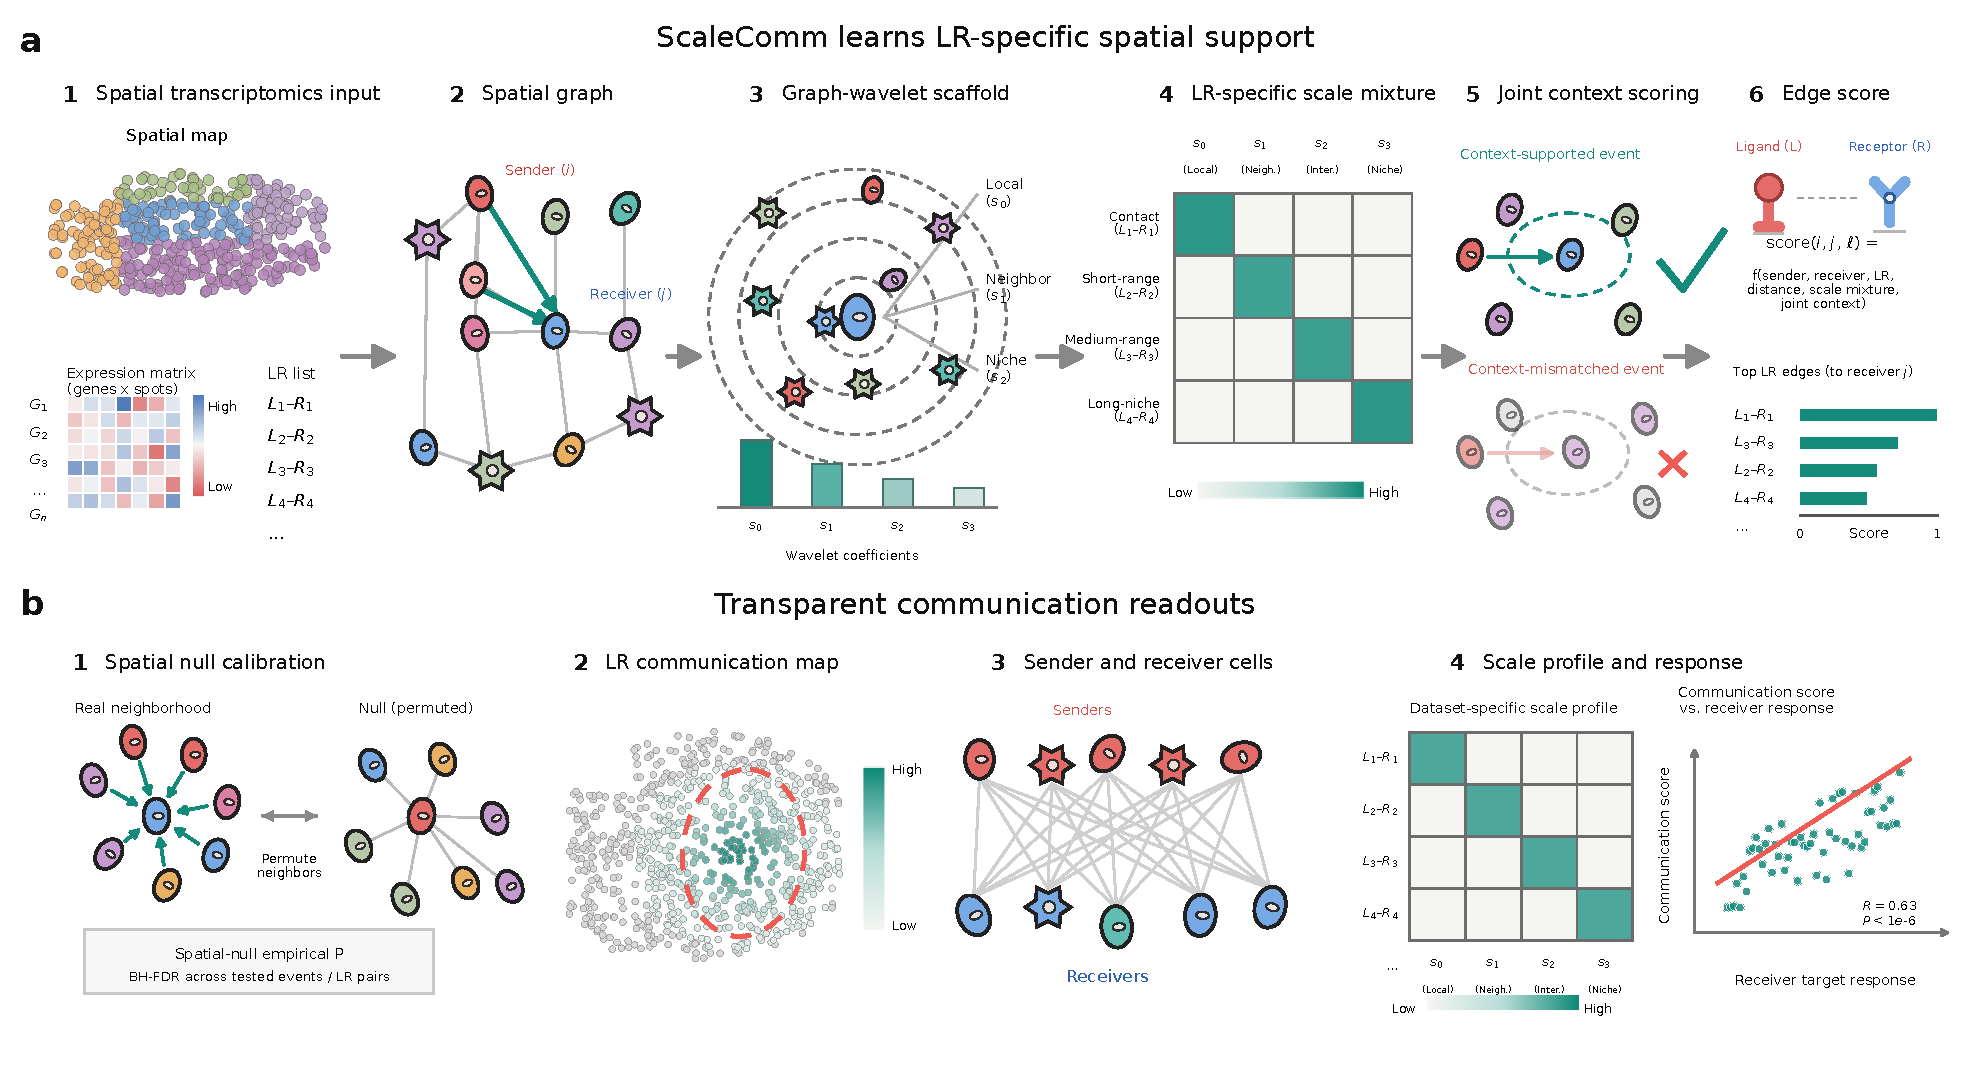
\includegraphics[width=\textwidth,height=0.72\textheight,keepaspectratio]{fig1_method_overview.pdf}
\caption{\textbf{ScaleComm framework for ligand-receptor-specific spatial support learning.}
\textbf{a,} Overview of the ScaleComm workflow. Spatial transcriptomics data are represented on a spatial graph that serves as a tissue scaffold, not as a fixed communication graph. Graph-wavelet features summarize localized multi-scale spatial support, and LR-specific scale mixtures with joint sender-receiver context features score candidate sender-receiver-LR events.
\textbf{b,} Main ScaleComm outputs, including spatial-null calibrated communication maps, sender and receiver event localization, LR-level rankings, inspectable LR-specific scale profiles and receiver-response validation readouts.}
\label{fig:method_overview}
\end{figure}
\FloatBarrier

\subsection{A mechanism-aware benchmark evaluates range-matched event recovery}

We next asked whether a method could recover not only the correct LR pair, but also the correct sender-receiver events for the intended spatial mechanism. Standard LR-pair AUPR or AUROC can be high even when a method assigns a plausible LR pair to the wrong spatial range or the wrong tissue niche. We therefore constructed a controlled semi-synthetic benchmark to complement, rather than replace, standard LR recovery evaluations (Fig.~\ref{fig:benchmark}a).

The benchmark used scDesign3-derived expression backgrounds fitted to lymph-node and melanoma references while retaining source spatial coordinates, local density, cell-type composition and tissue-domain annotations from the corresponding spatial templates \citep{scdesign3}. We then injected 200 LR programs with known event-level ground truth in each reference tissue: 120 positive LR programs evenly split across contact, short-range, medium-range and long-niche modes (30 per mode), and 80 hard-negative LR programs. The hard negatives stressed three failure modes: expression-driven false positives, wrong-niche calls and wrong-context sender-receiver rules (40 high-expression non-communication controls, 20 wrong-niche long-range controls and 20 wrong-context medium-range controls). For positive LR programs, the range-stress candidate space also included same-LR events outside the intended distance support, allowing wrong-range false-positive rates to be measured directly. Here, long-niche denotes broader spatial support restricted to a compatible tissue niche, not unrestricted long-distance diffusion.

We evaluated ScaleComm together with COMMOT, SpaOTsc, CellPhoneDB, CellChat, NICHES, SpaTalk, CellNEST and DeepTalk. All methods were run on the same benchmark inputs, and event-level comparisons used a common selected-candidate budget defined as the top 5\% ranked candidate events per tissue/noise setting for each method. When a method produced cell-type-level rather than event-level scores, its output was projected onto compatible candidate events. We therefore interpret projected event-level results for these methods as approximate localization analyses, while LR-level summaries provide their primary comparison. We report both event-level metrics, which evaluate localization of sender-receiver-LR triples, and LR-level summaries, which evaluate pair prioritization. In particular, top-$k$ precision refers to the precision among the top 100 ranked candidate events, whereas event-level precision and empirical FDR are computed at the fixed top-5\% candidate budget.

Across six tissue/noise settings, including clean, low-noise and high-noise versions of the two reference tissues, ScaleComm showed the most balanced performance at the common candidate budget. Values are reported descriptively as mean $\pm$ s.d. across these six settings. Because this benchmark evaluates event-level localization in a large candidate space rather than LR-pair ranking alone, absolute AUPR values are expected to be lower than in LR-level recovery tasks. Mean AUPR was 0.514 $\pm$ 0.116, compared with 0.372 $\pm$ 0.119 for COMMOT, the strongest non-ScaleComm baseline by AUPR. Mean AUROC was 0.829 $\pm$ 0.092, top-100 candidate precision was 0.772 $\pm$ 0.122 and event-level precision at the top-5\% budget was 0.648 $\pm$ 0.128. Specificity was high for all methods because the event space contains many negatives; therefore, the specificity panel is shown on an expanded scale, where ScaleComm reached 0.979 $\pm$ 0.005.

False-positive analyses showed a main advantage of the mechanism-aware design. ScaleComm had a lower empirical FDR than the strongest spatial baselines at the same candidate budget (0.352 $\pm$ 0.128 for ScaleComm versus 0.515 $\pm$ 0.155 for COMMOT) and selected few high-expression decoy events (0.002 $\pm$ 0.002). Wrong-range false-positive rates were low for ScaleComm (0.024 $\pm$ 0.012) and CellNEST (0.025 $\pm$ 0.014), but CellNEST recovered fewer positives in this benchmark (recall 0.048 $\pm$ 0.030 versus 0.287 $\pm$ 0.179 for ScaleComm), illustrating a precision-recall trade-off rather than a uniform ranking across all metrics. CellPhoneDB showed the highest weak-signal recall (0.287 $\pm$ 0.220 versus 0.115 $\pm$ 0.063 for ScaleComm), but this was accompanied by a higher wrong-range false-positive rate in the projected event evaluation (0.479 $\pm$ 0.156 versus 0.024 $\pm$ 0.012). Thus, the main conclusion from this benchmark is not that one method is best on every individual statistic, but that ScaleComm provides a favorable balance between LR recovery, event localization and suppression of mechanism-mismatched decoys.

The range-specific panels supported the value of LR-specific scale learning. Contact signals were the easiest for ScaleComm to recover (AUPR 0.776 across settings), whereas medium-range and long-niche programs were more sensitive to wrong-range and wrong-niche calls. ScaleComm retained informative recovery for medium-range and long-niche programs (AUPR 0.541 and 0.594, respectively) while keeping wrong-range rates low for medium-range events (0.003) and bounded for long-niche events (0.067). By comparison, long-niche wrong-range rates were higher for COMMOT and SpaOTsc (0.546 and 0.647, respectively), consistent with the difficulty of separating broader niche support from short-range co-expression patterns. As expected, adding noise reduced AUPR, but ScaleComm remained higher than the strongest non-ScaleComm baseline across the clean, low-noise and high-noise summaries (Fig.~\ref{fig:benchmark}d, g, h). Together, the benchmark separates LR-pair recovery from range-matched event recovery and shows that ScaleComm is most useful when high expression, spatial range and tissue context must be distinguished.

\begin{figure}[!p]
\centering
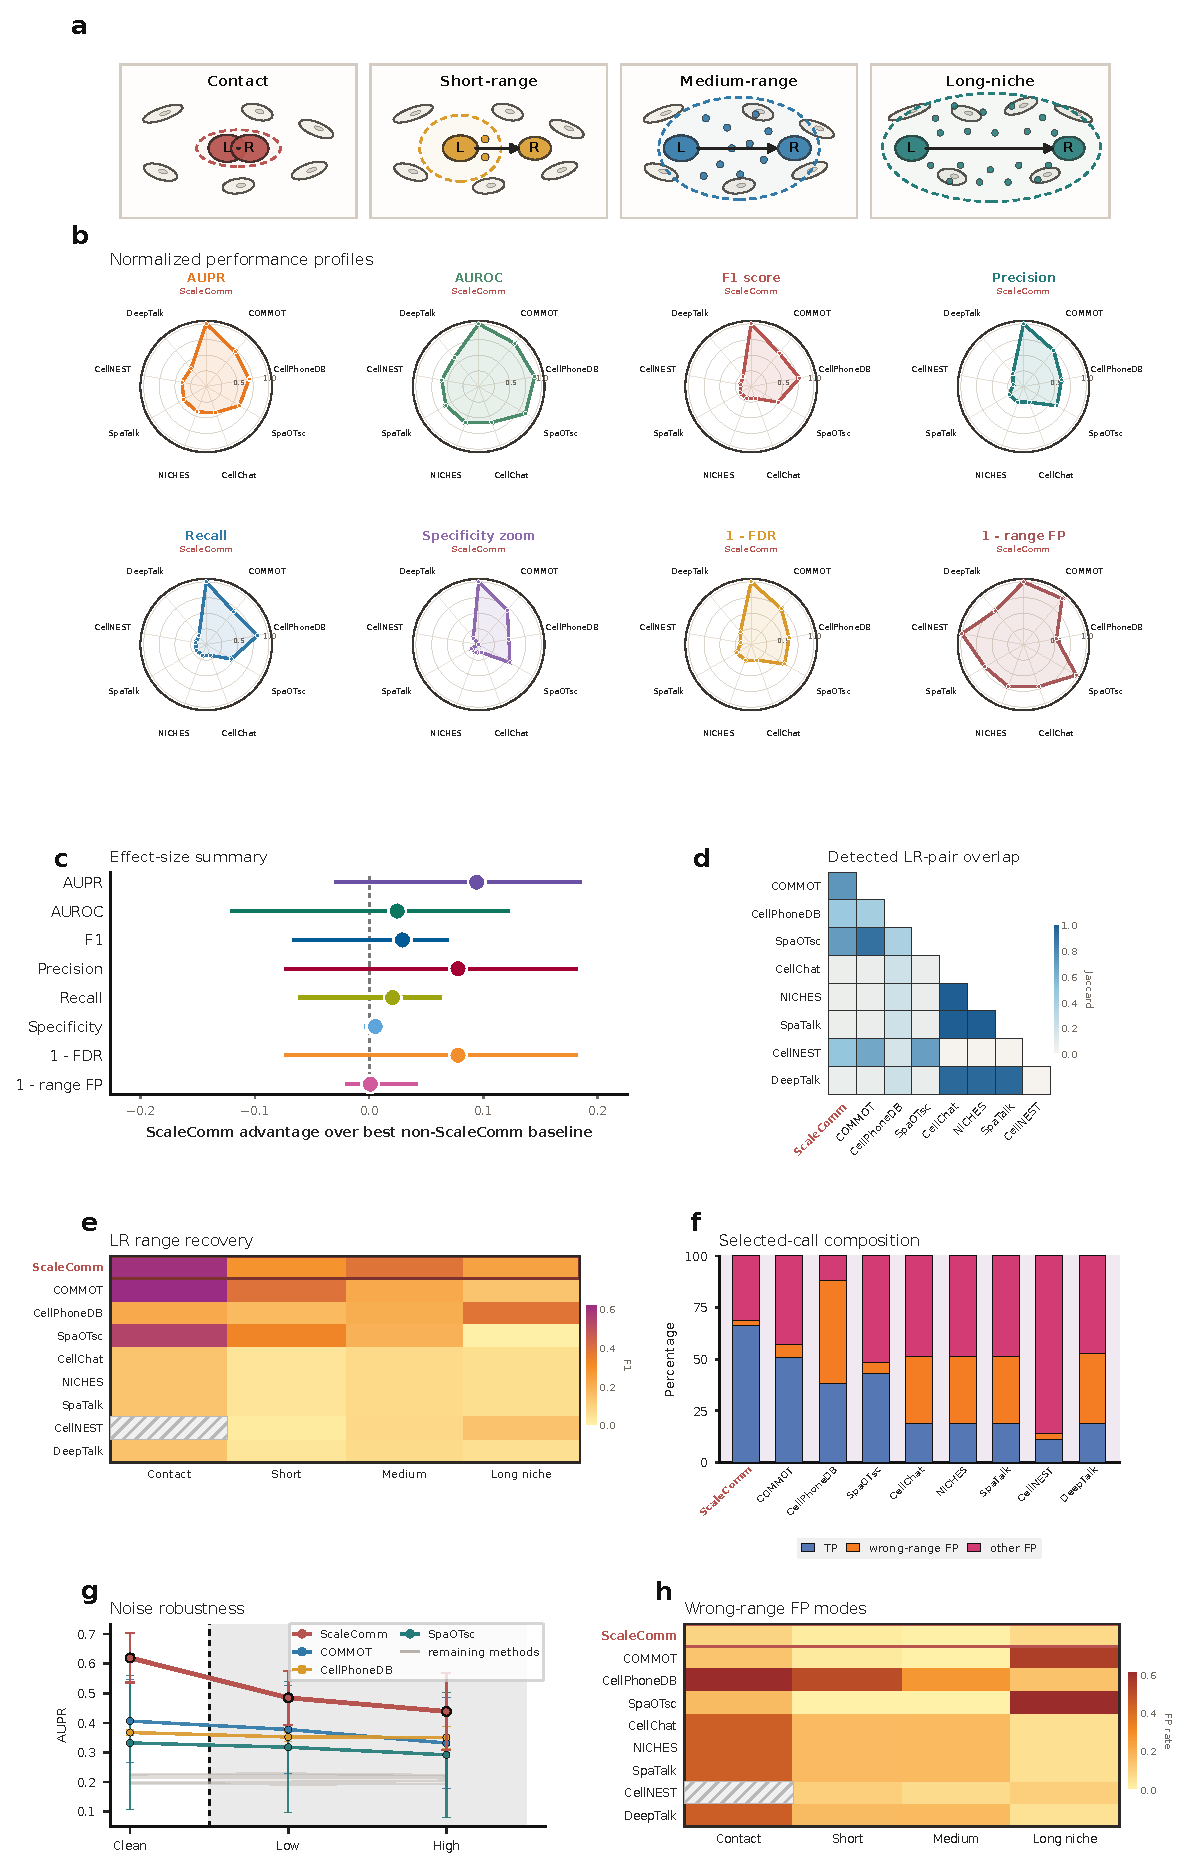
\includegraphics[width=\textwidth,height=0.72\textheight,keepaspectratio]{fig2_benchmark.pdf}
\caption{\textbf{Mechanism-aware benchmark for spatial communication inference.}
\textbf{a,} Benchmark design with four operational LR communication modes: contact, short-range, medium-range and long-niche communication. Long-niche denotes broader tissue-niche support rather than unrestricted long-distance diffusion.
\textbf{b,} Overall comparison showing recovery, precision, FDR and wrong-range false-positive control at a common selected-candidate budget.
\textbf{c,} Effect-size summary for key performance measures.
\textbf{d,} LR range recovery across communication modes.
\textbf{e,} Method overlap in detected LR pairs.
\textbf{f,} Composition of selected calls by communication mode and decoy class.
\textbf{g,} Robustness of benchmark performance under increasing noise.
\textbf{h,} Wrong-range false-positive patterns across methods.}
\label{fig:benchmark}
\end{figure}
\FloatBarrier

\subsection{ScaleComm localizes TGFB1-TGFBR2 candidate events in Visium HD colorectal cancer}

We next asked whether event-level scoring could localize a disease-relevant candidate communication program in high-resolution human tissue. We analyzed a Visium HD colorectal cancer section containing 6,000 spatial bins with tumor, stromal, myeloid, endothelial and lymphoid proxy annotations. Because TGF-beta signaling is closely linked to stromal activation, immune modulation and extracellular matrix remodeling in colorectal tumors \citep{massague2008tgfb,calon2012tgfb,calon2015stroma,guinney2015crc,tauriello2018tgfb,mariathasan2018tgfb}, we focused on TGFB1-TGFBR2 as a test case for whether a spatial candidate-event map aligns with a downstream receiver-state program rather than with ligand-receptor co-expression alone (Fig.~\ref{fig:crc_visium_hd}a).

TGFB1-TGFBR2 was among the most abundant LR axes in the tumor-stromal boundary, with 684 high-scoring top-edge receivers, ranking second among the displayed programs after CXCL12-CXCR4 (759 top-edge receivers; Fig.~\ref{fig:crc_visium_hd}b). Importantly, a simple expression-distance prior did not explain this prioritization. High-expression controls such as ACTB-KRT8 and COL1A1-EPCAM had substantially larger mean prior scores than TGFB1-TGFBR2 (0.00225 and 0.00189 versus $6.4 \times 10^{-5}$), indicating that ScaleComm was not merely selecting globally high-expression gene pairs (Fig.~\ref{fig:crc_visium_hd}c, d). The top 20\% TGFB1-TGFBR2 receiver map contained 1,200 bins and was enriched at tumor-immune, tumor-myeloid and tumor-stromal boundaries (29.6\%, 26.6\% and 18.0\% of top receivers, respectively). At the cell-proxy level, SPP1 macrophage, myeloid and CAF proxy bins accounted for 26.6\%, 21.2\% and 18.0\% of top receivers, respectively, consistent with a stromal-immune remodeling context.

We then evaluated whether the inferred TGFB1-TGFBR2 receiver map was supported by a downstream response program. A 13-gene TGF-beta/ECM response signature, excluding the ligand and receptor genes themselves, identified 200 response-hotspot bins with substantially higher target activity than the remaining tissue (mean 0.793 versus 0.149; Fig.~\ref{fig:crc_visium_hd}f). ScaleComm receiver scores were enriched in these response-hotspot bins (AUC 0.607, one-sided Mann-Whitney $P=8.17 \times 10^{-8}$). Across all 6,000 receivers, the receiver score showed a modest but significant correlation with the response signature (Spearman $\rho=0.143$, 95\% CI 0.118--0.166, $P=7.99 \times 10^{-29}$), larger than the corresponding COMMOT and CellNEST receiver summaries in this analysis (Spearman $\rho=0.037$ and 0.031, respectively; Fig.~\ref{fig:crc_visium_hd}g--j). These comparisons are not intended as a full real-data benchmark, because the methods produce different output layers, but they show that the ScaleComm event map is more closely aligned with an independent receiver-state readout in this CRC section. Sender-receiver layer maps further separated putative sending and receiving bins across the tumor, myeloid and stromal compartments, with the strongest cell-type-pair counts involving SPP1 macrophage, myeloid, CAF and tumor proxy compartments (Fig.~\ref{fig:crc_visium_hd}k, l).

\begin{figure}[!p]
\centering
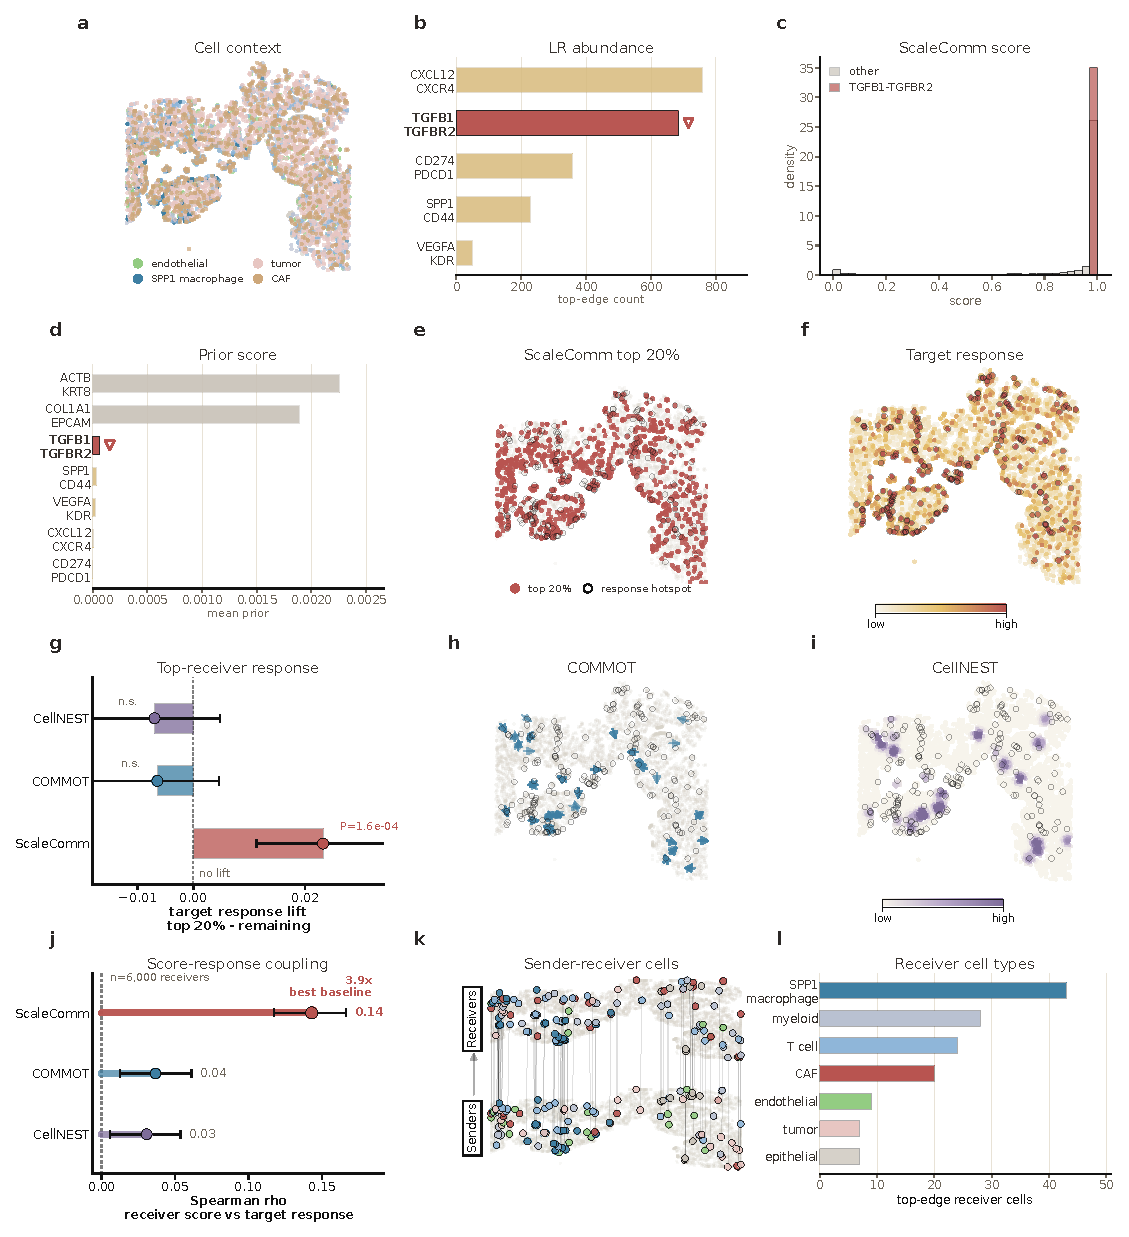
\includegraphics[width=\textwidth,height=0.72\textheight,keepaspectratio]{fig3_crc_visium_hd.pdf}
\caption{\textbf{ScaleComm localizes TGFB1-TGFBR2 candidate events in Visium HD colorectal cancer.}
\textbf{a,} Cell and niche context for the analyzed Visium HD CRC section.
\textbf{b,} LR abundance among high-scoring receiver events in the tumor-stromal boundary.
\textbf{c,} ScaleComm score distribution for TGFB1-TGFBR2 relative to other LR and control gene-pair candidates.
\textbf{d,} Expression-distance prior scores for LR and high-expression control gene pairs.
\textbf{e,} Top 20\% ScaleComm TGFB1-TGFBR2 receiver map.
\textbf{f,} TGF-beta/ECM downstream response signature map.
\textbf{g,} Target-response enrichment among top receivers.
\textbf{h, i,} COMMOT and CellNEST receiver maps shown as reference visualizations for the same LR axis.
\textbf{j,} Correlation between receiver score and downstream response across 6,000 receivers.
\textbf{k,} Sender and receiver layers for top TGFB1-TGFBR2 events.
\textbf{l,} Cell-type-pair summary of top sender-receiver events.}
\label{fig:crc_visium_hd}
\end{figure}
\FloatBarrier

\subsection{ScaleComm resolves stage-associated programs in mouse colon inflammation}

We next asked whether the same event-level framework could summarize stage-associated differences in communication programs during inflammation and tissue remodeling. We analyzed a mouse colon MERFISH DSS time course spanning healthy D0, acute D3, inflammatory D9 and later D21 states, with 900 cells summarized per stage into epithelial, immune, mesenchymal, vascular and neural compartments (Fig.~\ref{fig:dss_merfish}a). Because this experiment is cross-sectional rather than a lineage-traced time series, we interpret the results as stage-associated communication programs rather than causal temporal trajectories.

ScaleComm recovered distinct LR activity programs across the four stages. A homeostatic program was highest at D0, an early-response program peaked at D3, an inflammatory-peak program peaked at D9 and a repair/remodeling program peaked at D21 after max-normalization within each program (Fig.~\ref{fig:dss_merfish}d). The LR composition of local high-scoring events matched this stage structure. At D9, the local inflammatory list included Cxcl2-Cxcr1 (60 local edges), Cxcl10-Cxcr3 (58), Cxcl2-Cxcr2 (55), Il1b-Il1r2 (37) and Il1b-Il1r1 (32), consistent with chemokine and IL-family communication in the acute inflammatory compartment. At D21, the local list shifted toward Cx3cl1-Cx3cr1 (60), Cxcl12-Ackr3 (50), Cxcl12-Cxcr4 (42), Tgfb3-Acvrl1 (19) and Wnt10a-Fzd1 (17), consistent with a later remodeling or repair-associated state (Fig.~\ref{fig:dss_merfish}c, k, m).

The stage-specific patterns were not reducible to one dominant LR pair. Across the LR shift landscape, inflammatory axes such as Il1b-Il1r2 rose from D0 to D9 (0.504 to 0.980 in normalized activity), whereas repair-associated axes such as Cxcl12-Cxcr4 were retained in the D21 local program (Fig.~\ref{fig:dss_merfish}g, m). D9 compartment-flow summaries showed epithelial-centered communication with immune and vascular involvement, and the D9 receiver-burden map localized cells receiving multiple high-scoring inflammatory events rather than only a single LR axis (Fig.~\ref{fig:dss_merfish}h, i). Local zoom maps further showed that selected D9 and D21 events occupied restricted tissue regions rather than the entire section (Fig.~\ref{fig:dss_merfish}j, l). Replicate agreement for top LR lists was moderate, with Jaccard overlap ranging from 0.33 to 0.54 across stages, which is consistent with biological and sampling heterogeneity across DSS sections (Fig.~\ref{fig:dss_merfish}f). Together, these analyses indicate that ScaleComm can summarize a spatial inflammation time course as coordinated, stage-associated communication programs while preserving the local LR events underlying each program.

\begin{figure}[!p]
\centering
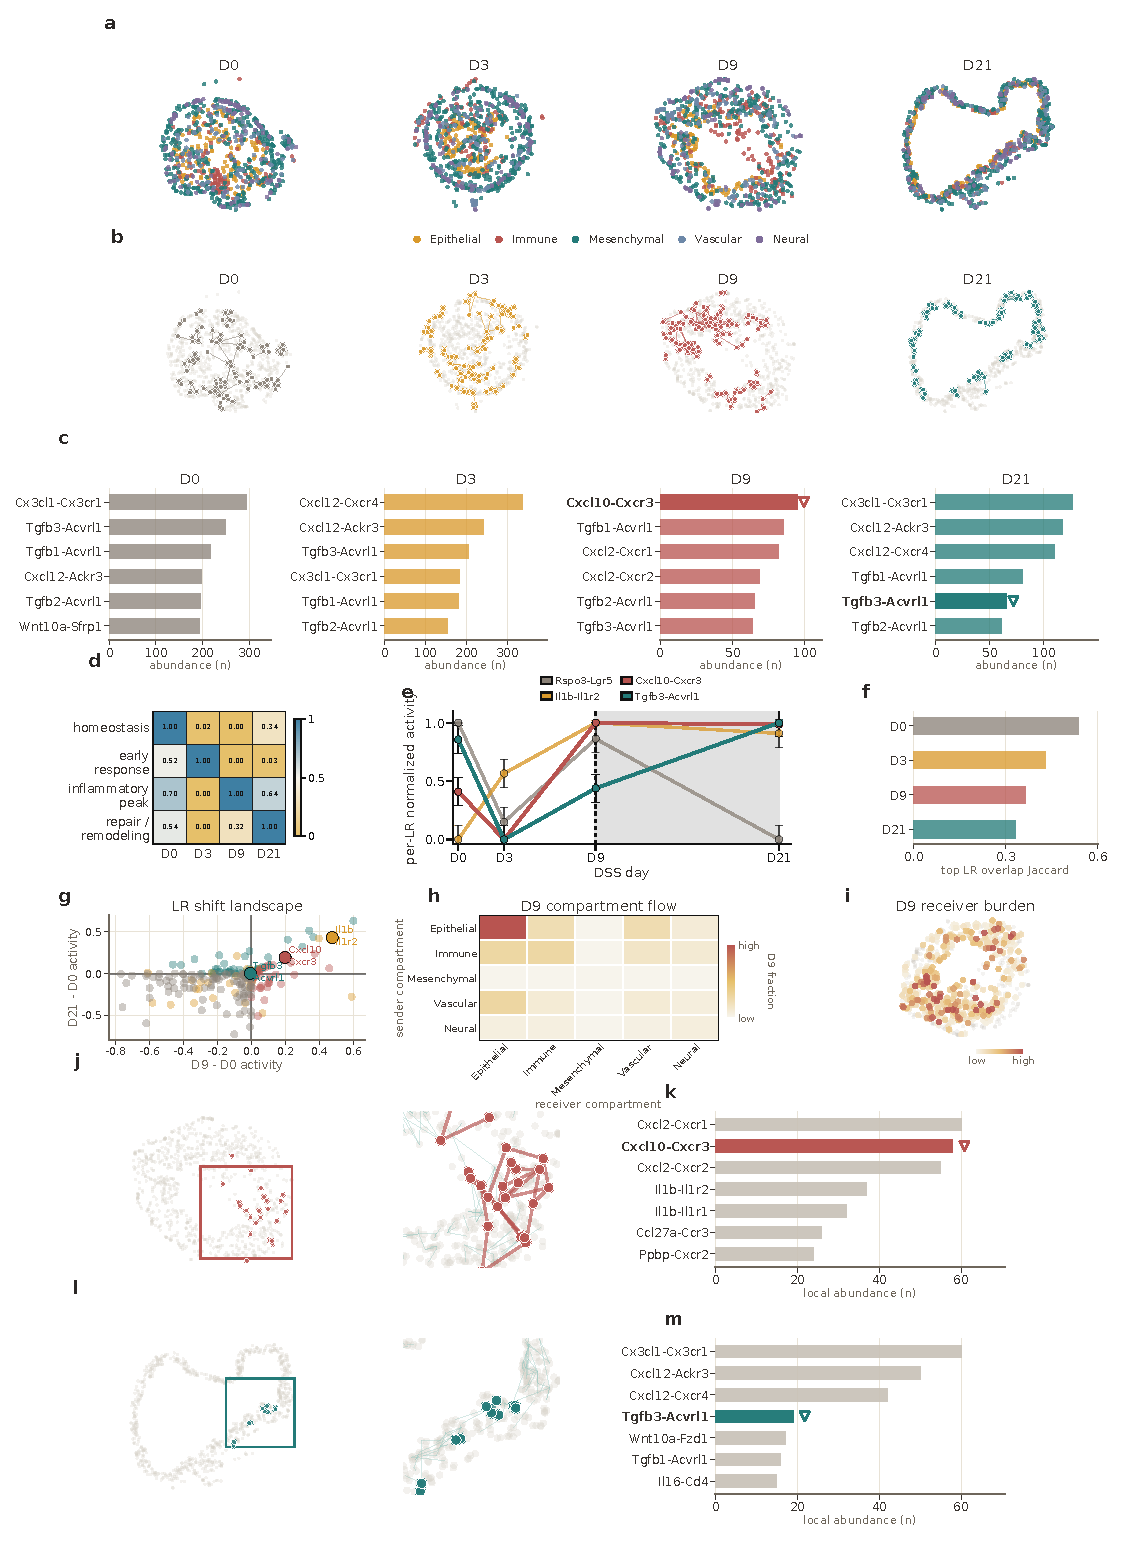
\includegraphics[width=\textwidth,height=0.72\textheight,keepaspectratio]{fig4_dss_merfish.pdf}
\caption{\textbf{ScaleComm resolves stage-associated communication programs in mouse colon DSS inflammation.}
\textbf{a,} Compartment composition across healthy D0 and DSS D3, D9 and D21 stages.
\textbf{b,} Stage-specific high-scoring communication-region summaries based on aggregated receiver activity.
\textbf{c,} Top LR abundance profiles across stages.
\textbf{d,} Max-normalized activity of homeostatic, early-response, inflammatory-peak and repair/remodeling programs.
\textbf{e,} Representative LR activity trajectories.
\textbf{f,} Replicate consistency of top LR lists.
\textbf{g,} LR shift landscape comparing D9 and D21 activity relative to D0.
\textbf{h,} D9 compartment-level sender-receiver flow.
\textbf{i,} D9 receiver burden map.
\textbf{j, l,} Zoomed maps of local D9 inflammatory and D21 repair/remodeling events.
\textbf{k, m,} Local LR abundance rankings for D9 and D21.}
\label{fig:dss_merfish}
\end{figure}
\FloatBarrier

\subsection{ScaleComm estimates context-specific scale profiles in CosMx non-small cell lung cancer}

The benchmark results suggested that LR-specific scale learning and joint sender-receiver context features can help suppress mechanism-mismatched events. We therefore asked whether these model components produce inspectable and response-supported programs in real single-cell spatial data. We analyzed a CosMx non-small cell lung cancer field of view containing 9,000 cells, with tumor, T-cell, myeloid, stromal, endothelial and immune proxy annotations distributed across vascular-stromal, tumor-myeloid, stromal-immune and tumor-immune interfaces (Fig.~\ref{fig:cosmx_nsclc}a).

The estimated scale profiles did not collapse to a single preferred range across LR pairs. In this dataset, CCL5-CCR5 was strongly local-biased (local weight 0.978), SPP1-CD44 showed an intermediate-scale profile, and ScaleComm assigned broader-support profiles to CXCL12-CXCR4 and VEGFA-KDR (broad weights 0.976 and 0.946, respectively; Fig.~\ref{fig:cosmx_nsclc}b, c). These profiles should be interpreted as dataset-specific effective supports, not as fixed molecular diffusion ranges. For example, CXCL12-CXCR4 ranked highest by mean ScaleComm score, with 316 top events, a median top-event distance of 166 microns and 84.2\% of top events located in the stromal-immune interface. By contrast, TGFB1-TGFBR2 had a shorter median top-event distance of 75 microns and a broader tumor-stromal or vascular-stromal response context. This pattern illustrates why a single neighborhood radius would be difficult to justify for all LR axes in the same field of view.

Receiver-response analyses provided a second check on the estimated profiles. CXCL12-CXCR4 had the strongest receiver score-response correlation among the candidate axes (Spearman $\rho=0.457$), while several additional LR axes showed elevated target response in top receivers, including CSF1-CSF1R, VEGFA-KDR, TGFB1-TGFBR2, CXCL10-CXCR3 and CCL5-CCR5 (target-response lifts of 0.603, 0.368, 0.214, 0.210 and 0.200, respectively; Fig.~\ref{fig:cosmx_nsclc}e, f). Comparing the scale-aware model with a no-scale variant showed that scale-aware scoring increased target Spearman correlation for several, but not all, LR axes: CXCL12-CXCR4 improved by 0.117, CXCL9-CXCR3 by 0.065, CXCL10-CXCR3 by 0.053, VEGFA-KDR by 0.049 and SPP1-CD44 by 0.016 (Fig.~\ref{fig:cosmx_nsclc}i). Other axes, including CD274-PDCD1, CSF1-CSF1R and CCL5-CCR5, were not improved by this comparison. We interpret this as evidence that LR-specific scale mixtures are useful for a subset of context-dependent axes in this dataset, rather than as a claim that scale learning uniformly improves every LR pair. The receiver cell-type burden and spatial maps further show that the selected programs converge on T-cell-enriched receiver states within vascular-stromal and stromal-immune interfaces (Fig.~\ref{fig:cosmx_nsclc}g, h).

\begin{figure}[!p]
\centering
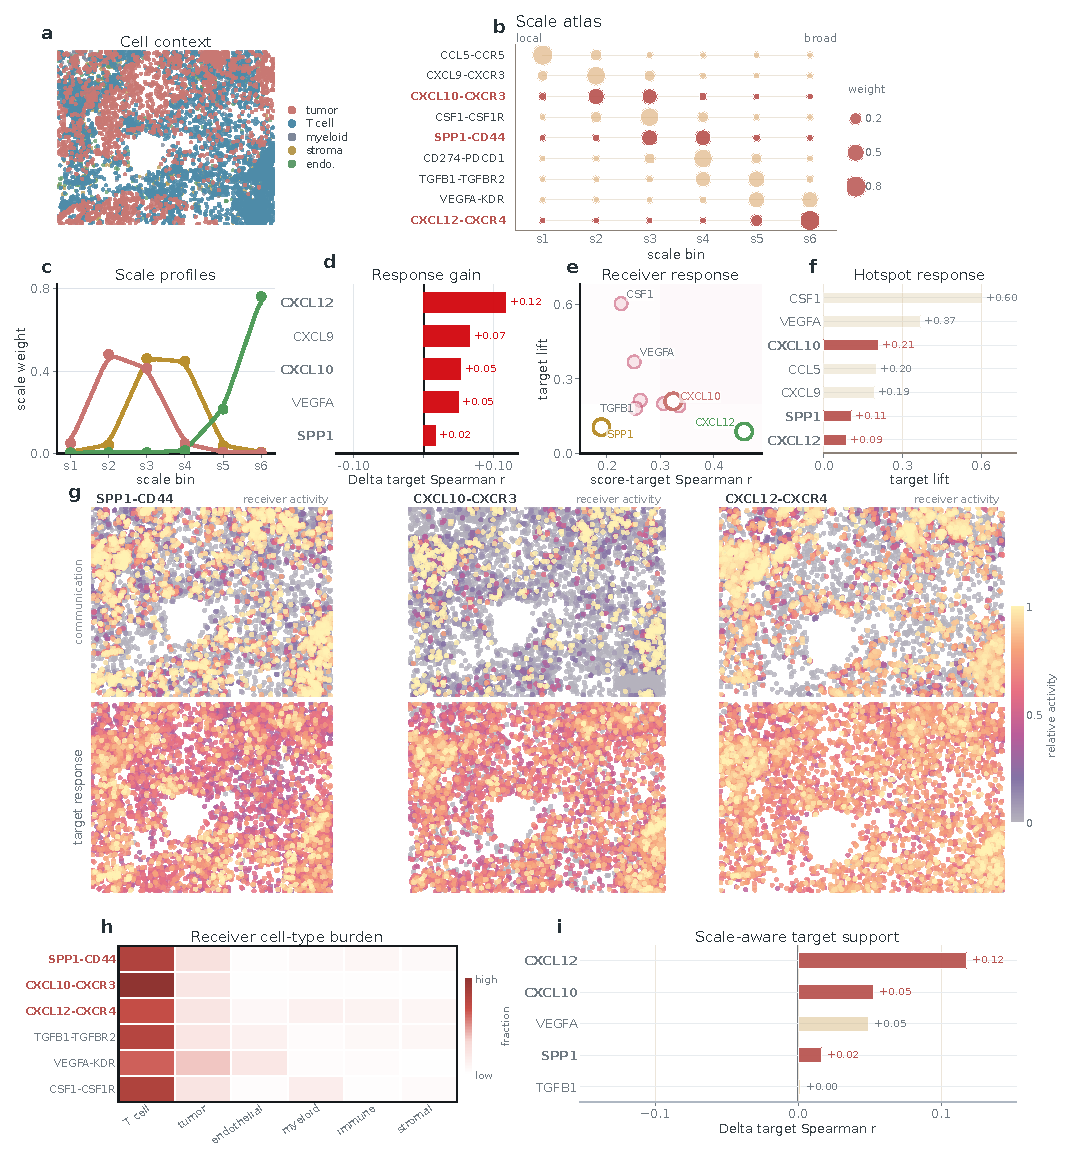
\includegraphics[width=\textwidth,height=0.72\textheight,keepaspectratio]{fig5_cosmx_nsclc.pdf}
\caption{\textbf{ScaleComm estimates context-specific scale profiles in CosMx NSCLC.}
\textbf{a,} Cell and tissue-context map for the analyzed 9,000-cell CosMx NSCLC field of view.
\textbf{b,} LR-specific scale profiles across candidate immune, stromal and angiogenic communication axes.
\textbf{c,} Scale-profile traces showing local, intermediate and broad effective support patterns.
\textbf{d,} Target-response gain for selected LR programs.
\textbf{e,} Receiver-response support for selected LR axes.
\textbf{f,} Target-response lift in top receiver cells.
\textbf{g,} Spatial receiver-activity and target-response maps for representative communication programs.
\textbf{h,} Receiver cell-type burden across selected LR programs.
\textbf{i,} Change in receiver score-response correlation for the scale-aware model relative to a no-scale variant.}
\label{fig:cosmx_nsclc}
\end{figure}
\FloatBarrier

\subsection{ScaleComm localizes a CXCL13-CXCR5 germinal-center program in tonsil data}

Finally, we asked whether ScaleComm could recover a canonical spatial chemokine program in organized lymphoid tissue. We analyzed SPAMOSAIC tonsil sections with B-cell, FDC, T-cell, Tfh, myeloid, stromal and epithelial proxy annotations. In the displayed A1 section, 862 of 2,500 spatial units were assigned to a germinal-center proxy region, providing a clear tissue context for evaluating CXCL13-CXCR5 candidate events (Fig.~\ref{fig:tonsil_spamosaic}a, b).

The top 300 CXCL13-CXCR5 receiver units were strongly enriched in the germinal-center proxy region. In A1, 242 of 300 top receivers were in the germinal-center proxy region, compared with 862 of 2,500 units in the background (80.7\% versus 34.5\%; fold enrichment 2.34; Fisher one-sided $P=5.40 \times 10^{-54}$). Top receivers were dominated by B-cell and FDC proxy annotations (37.3\% and 35.3\%), with additional Tfh proxy contribution (8.0\%; Fig.~\ref{fig:tonsil_spamosaic}c, e). A 12-gene B-cell/GC response signature was elevated in top receivers, with a top-versus-background response lift of 0.807 and a receiver score-response Spearman correlation of 0.622 ($P=6.69 \times 10^{-81}$; Fig.~\ref{fig:tonsil_spamosaic}d, f).

The pattern was reproduced in a second section. In D1, 81.7\% of the top 300 CXCL13-CXCR5 receivers were in the germinal-center proxy region compared with 36.2\% of background units, giving a 2.25-fold enrichment; the receiver score-response correlation remained high (Spearman $\rho=0.594$, $P=1.08 \times 10^{-71}$; Fig.~\ref{fig:tonsil_spamosaic}i). Although CXCL13-CXCR5 was not the strongest axis by global mean score, it ranked second by the number and fraction of top-20\% LR hotspot receivers within the germinal-center region in both A1 and D1 (367 of 500 and 392 of 500 top-20\% receivers in GC, respectively; Fig.~\ref{fig:tonsil_spamosaic}g). This distinction is important: the result supports local GC-enriched communication rather than a tissue-wide high-expression LR ranking. Sender-receiver summaries further localized top CXCL13-CXCR5 events among FDC-to-FDC, FDC-to-B-cell, myeloid-to-B-cell and B-cell-to-B-cell pairs. As a visualization layer, the same prediction table was also exported to an interactive browser for inspecting LR maps, sender-receiver pairs and cell-type filters (Fig.~\ref{fig:tonsil_spamosaic}h, j, k).

\begin{figure}[!p]
\centering
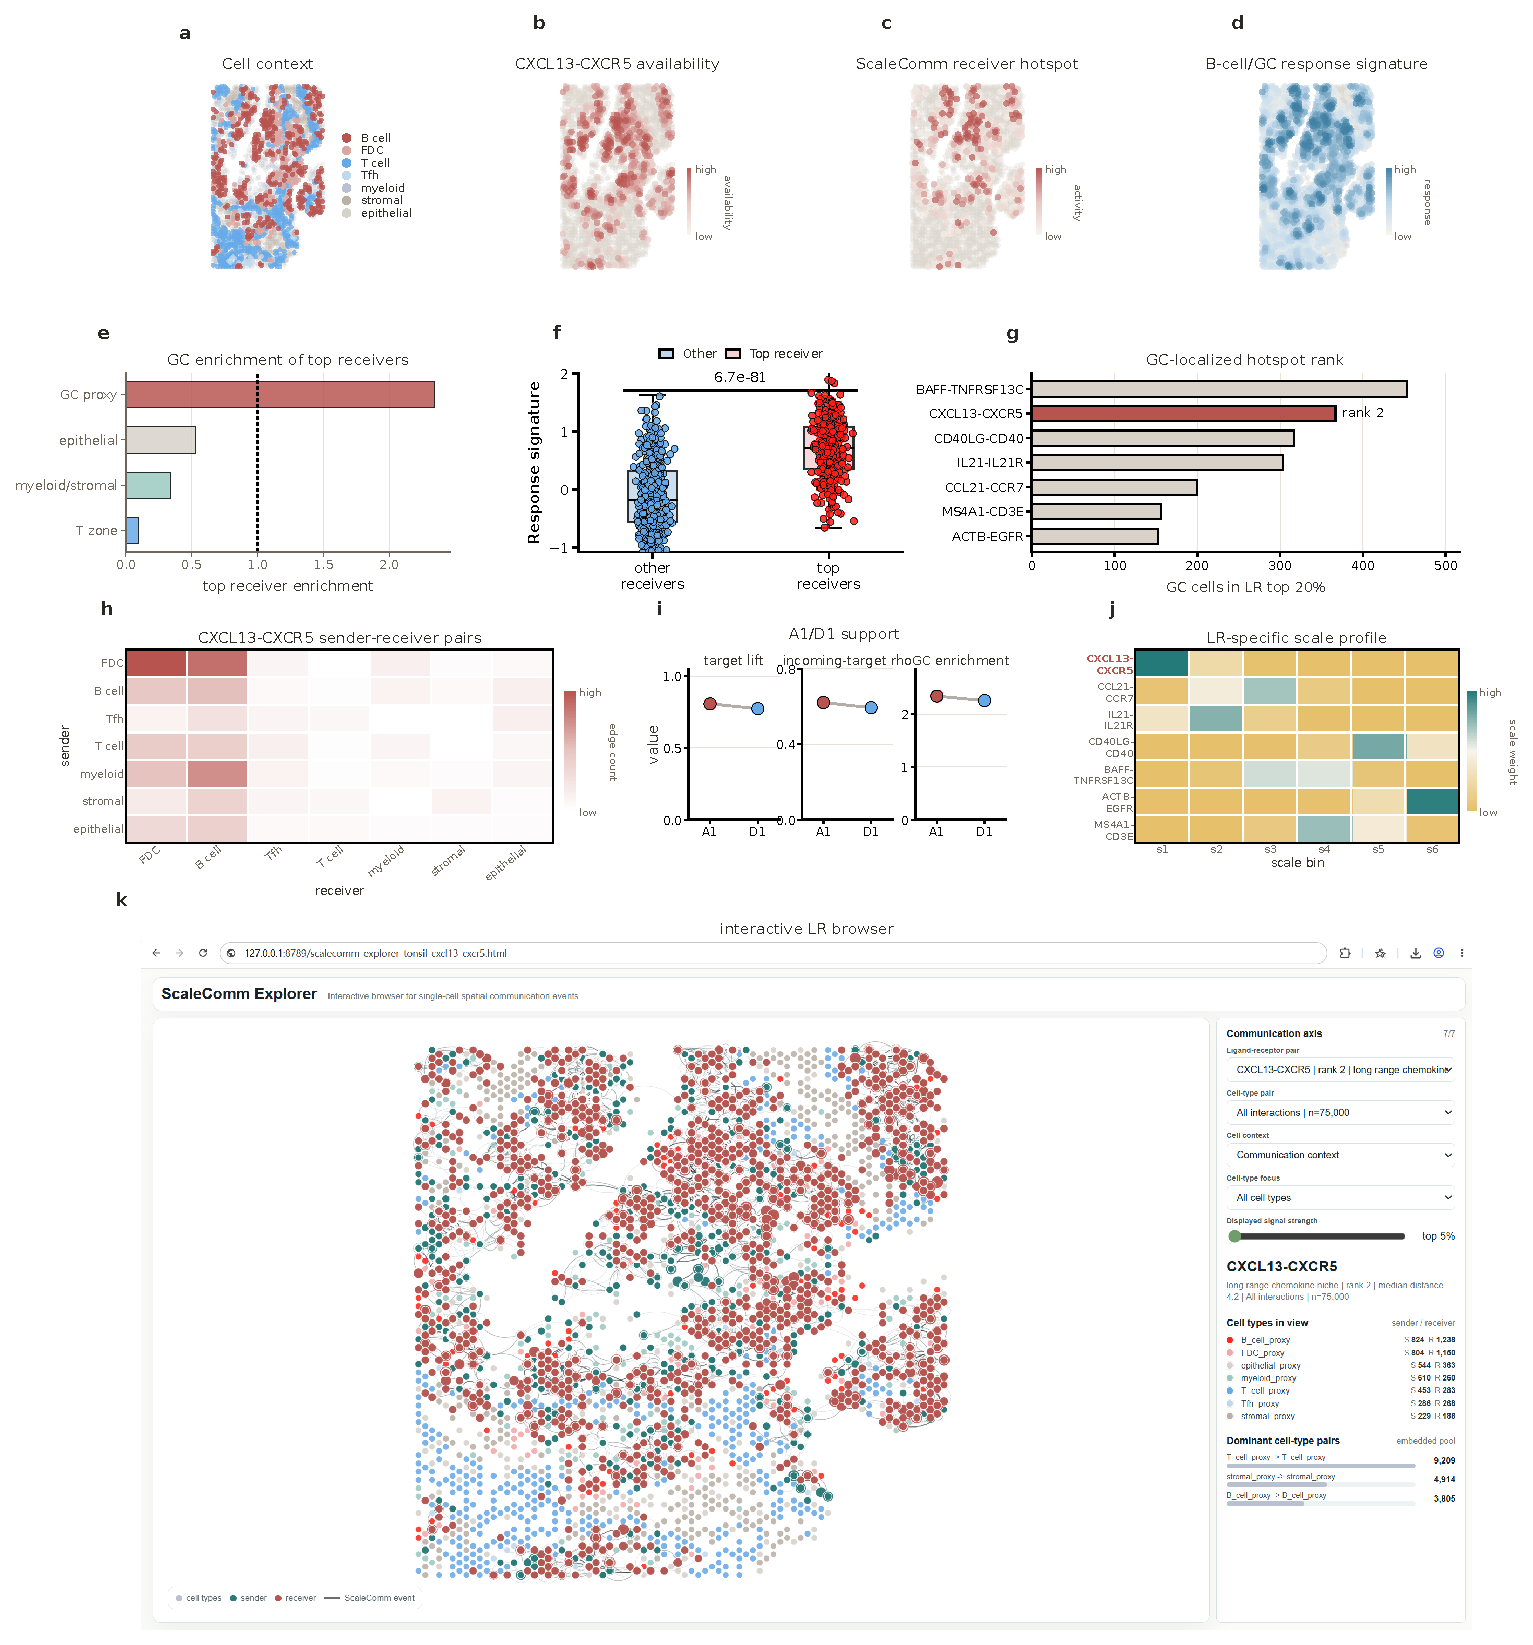
\includegraphics[width=\textwidth,height=0.72\textheight,keepaspectratio]{fig6_tonsil_spamosaic.pdf}
\caption{\textbf{ScaleComm localizes CXCL13-CXCR5 communication to the germinal-center context in tonsil data.}
\textbf{a,} Cell-context map for the analyzed SPAMOSAIC tonsil section.
\textbf{b,} CXCL13 and CXCR5 availability across the section.
\textbf{c,} ScaleComm CXCL13-CXCR5 receiver hotspot map.
\textbf{d,} B-cell/GC downstream response signature map.
\textbf{e,} Germinal-center and cell-type enrichment among top receivers.
\textbf{f,} Response signature distribution in top receivers and other receivers.
\textbf{g,} GC-localized top-20\% LR hotspot counts.
\textbf{h,} CXCL13-CXCR5 sender-receiver pair summary.
\textbf{i,} Replicate support across A1 and D1 sections.
\textbf{j,} LR-specific scale-profile display.
\textbf{k,} Interactive ScaleComm browser view used as a visualization layer for LR-level spatial inspection.}
\label{fig:tonsil_spamosaic}
\end{figure}
\FloatBarrier

\section{Discussion}\label{sec:discussion}

ScaleComm was developed around a specific problem in spatial CCC inference: the effective spatial support of a candidate communication event is LR-specific and tissue-context dependent. Rather than treating the nearest-neighbor graph as the communication graph itself, ScaleComm uses the graph as a scaffold for localized multi-scale summaries and lets each LR pair mix those supports when scoring candidate sender-receiver events. This design keeps spatial proximity in the model, but prevents proximity alone from being interpreted as signaling.

The mechanism-aware benchmark was designed to test this distinction directly. It does not replace standard LR-pair recovery metrics; instead, it asks whether a method can assign LR programs to the intended sender-receiver events and spatial modes. This is why several baselines performed well on selected metrics but showed different trade-offs. For example, CellNEST had low wrong-range false-positive rates in this benchmark but lower recall, whereas CellPhoneDB recovered more weak-signal LR programs after projection but also produced more wrong-range event calls. These trade-offs clarify why range-matched event recovery should be evaluated separately from ordinary LR-pair ranking. In this controlled setting, ScaleComm provided a favorable balance between event-level recovery, LR prioritization and suppression of high-expression or mechanism-mismatched decoys.

Across real datasets, we used receiver-response analyses, tissue-region enrichment and cell-type-pair summaries as supporting evidence rather than as definitive ground truth. In Visium HD CRC, TGFB1-TGFBR2 receiver events aligned with a TGF-beta/ECM response signature in tumor-stromal and tumor-myeloid contexts. In the DSS MERFISH time course, ScaleComm summarized stage-associated inflammatory and remodeling programs while preserving local LR events. In CosMx NSCLC, dataset-specific scale profiles differed across LR axes and scale-aware scoring improved receiver-response alignment for several, but not all, programs. In tonsil spatial data, CXCL13-CXCR5 receiver hotspots were strongly enriched in germinal-center proxy regions and reproduced across sections. These analyses support the practical value of localized candidate events and inspectable scale profiles, but they do not establish complete native CCC ground truth.

The dataset-specific scale profile should be interpreted carefully. It is an empirical support profile within a dataset and candidate universe, not a molecular diffusion constant. A broad profile may reflect ligand diffusion, aligned sender and receiver domains, tissue architecture, cell density or correlated downstream state. Similarly, high receiver-response correlation supports biological plausibility but remains an observational association. Perturbation experiments, temporal measurements and direct protein-level assays will be needed to establish causality for individual LR axes.

ScaleComm has several limitations. First, training uses pseudo-labels derived from expression, distance and tissue-context priors when native event-level labels are unavailable. The benchmark and hard-negative analyses test whether this supervision can recover known injected mechanisms, but the pseudo-label design remains a modeling assumption. Second, the current implementation treats LR pairs at the pair level and does not fully model multi-subunit receptor complexes or co-receptors. Third, output resolution depends on the spatial platform: a Visium HD bin, a MERFISH cell, a CosMx cell and a Slide-seq or SPAMOSAIC bead have different biological and technical meanings. Fourth, cell-type-level baselines require projection to event-level candidates for some comparisons, and those projected maps should be interpreted as approximate localization analyses. Finally, spatial-null calibration is a post hoc readout; it helps evaluate whether high scores exceed selected null distributions but does not by itself prove signaling.

Future extensions could incorporate explicit ligand-target priors during training, model multi-subunit complexes, add protein or chromatin measurements, and use temporal or perturbational spatial data to distinguish predicted communication from downstream consequence. The same event-level representation could also support interactive analysis tools, where users inspect LR maps, sender-receiver layers, cell-type filters and response signatures in a single tissue view. More broadly, we expect LR-specific spatial support to be useful as spatial transcriptomics moves toward larger cohorts, higher resolution and multi-modal tissue atlases.

\section{Conclusions}\label{sec:conclusions}

ScaleComm provides a graph-wavelet framework for event-level spatial CCC inference with LR-specific scale mixtures and dataset-specific scale profiles. By combining multi-scale spatial context, candidate sender-receiver scoring, spatial-null readouts and receiver-response validation, ScaleComm helps distinguish high ligand-receptor co-expression from mechanism-consistent communication hypotheses. The benchmark and cross-platform analyses support its use for nominating spatially localized LR programs that can be followed up with targeted biological validation.

\section{Methods}\label{sec:methods}

\subsection{Method overview}

ScaleComm takes as input an expression matrix $X \in \mathbb{R}^{n \times g}$, spatial coordinates $u_i \in \mathbb{R}^2$ for $n$ cells, spots or bins, optional cell or region annotations, and an LR catalogue. The output is a scored table of candidate sender-receiver-LR events. An event is a triple $(i,j,\ell)$, where $i$ is the candidate sender, $j$ is the candidate receiver and $\ell=(L_\ell,R_\ell)$ is an LR pair. Event-level scores can be aggregated to LR-pair rankings, sender-receiver cell-type-pair summaries, receiver burden maps or LR-specific hotspot maps.

The central modeling choice is to separate the tissue scaffold from the communication event. A spatial graph is built from tissue coordinates and used for graph-wavelet feature construction. Candidate communication events can include sender-receiver pairs beyond direct graph neighbors, depending on the dataset-specific candidate table. Thus, the K-nearest-neighbor graph defines the geometry over which local tissue state is summarized; it does not by itself define which cells or spots are allowed to communicate.

\subsection{Preprocessing and LR catalogue}

For each dataset, genes absent from the expression matrix were removed from the LR catalogue before scoring. When raw counts were available, expression matrices were library-size normalized and log-transformed; otherwise, processed expression values supplied with the dataset were used. These steps follow common single-cell and spatial transcriptomic analysis conventions implemented in widely used ecosystems such as Scanpy, Seurat, Tangram and cell2location \citep{scanpy2018,seurat2019,tangram2021,cell2location2022}. Features used by the neural model were standardized gene-wise within each analyzed section or benchmark replicate. Dataset-provided annotations were used when available. For datasets without final cell-type labels at the analyzed resolution, we used proxy labels derived from marker expression or upstream clustering, and interpreted cell-type-pair summaries as proxy summaries rather than definitive cell identities.

The LR universe was defined at the pair level. The current manuscript analyses do not explicitly resolve multi-subunit receptor complexes. Curated LR resources and downstream response signatures were assembled from public LR and pathway knowledge bases, including CellChatDB, CellPhoneDB, OmniPath and NicheNet where applicable \citep{cellchat2021,cellphonedb2020,omnipath2021,nichenet2020}. Ligand and receptor genes used directly to score an LR pair were excluded from downstream response signatures when evaluating receiver-state support.

\subsection{Datasets and source information}

All analyses used public or preprocessed spatial transcriptomic datasets converted into a common table format containing coordinates, expression, candidate LR pairs, candidate sender-receiver events and optional annotations. Dataset-specific metadata files were retained with the processed inputs and will be released with the code package.

The mechanism-aware benchmark used two semi-synthetic reference templates: a human lymph-node Visium template and a human melanoma spatial multiome template. scDesign3-derived expression backgrounds were generated from these templates and combined with retained source coordinates, local density, cell-type or region labels and injected LR programs \citep{scdesign3}. The benchmark data are controlled datasets generated for this study, not native CCC ground truth.

The CRC analysis used the public 10x Genomics Visium HD human colorectal cancer dataset from the P2CRC section, corresponding to GEO sample GSM8594568 and the Visium HD CRC study by Oliveira et al. \citep{oliveira2025visiumhdcrc}. We used the 8-\(\mu\)m binned expression matrix, spatial coordinates and published deconvolution or tissue-context metadata, then selected a 6,000-bin tumor, stromal, myeloid, endothelial and lymphoid enriched region of interest.

The mouse colon inflammation analysis used the Cadinu et al. mouse colon IBD MERFISH resource and the associated Dryad dataset \citep{cadinu2024colitis,moffitt2024dryad}. One representative slice was selected for each displayed stage: healthy D0, DSS D3, DSS D9 and DSS D21. Each stage-level table contained 900 cells, 990 expression genes, 260 LR pairs and the stage-specific candidate event table.

The CosMx analysis used the NanoString FFPE human non-small cell lung cancer CosMx SMI dataset distributed through \texttt{SFEData::HeNSCLCData} and ExperimentHub EH7743 \citep{he2022cosmx,sfedata2026}. The raw object contained 100,290 cells. We selected a 9,000-cell tumor, immune, stromal and interface-enriched subset with 39 exported genes, 11 LR pairs and 251,727 candidate events.

The tonsil analysis used processed SPAMOSAIC human tonsil RNA+ADT sections A1 and D1. For each section, we used spatial coordinates, RNA expression and ADT-derived proxy annotations from the processed h5ad files. Each section-level analysis used 2,500 spatial units, 49 exported expression genes, seven LR pairs and 525,000 candidate events. Because the region and cell-type labels are marker-derived proxy annotations, we interpret germinal-center and cell-type-pair summaries as proxy tissue-context evidence rather than curated histological ground truth.

\subsection{Spatial graph and graph-wavelet pyramid}

For each section or replicate, ScaleComm constructs an undirected K-nearest-neighbor graph from spatial coordinates. In the manuscript analyses, the default training graph used $K=12$ neighbors. Let $A$ denote the adjacency matrix with self-loops and $D$ its degree matrix. We use the symmetric normalized propagation operator
\begin{equation}
P = D^{-1/2} A D^{-1/2}.
\end{equation}
For diffusion steps $\mathcal{T}=\{1,2,4,8\}$, low-pass signals are computed as
\begin{equation}
H^{(t)} = P^t X,\quad t \in \mathcal{T}.
\end{equation}
Rather than using a full spectral eigendecomposition, ScaleComm uses a sparse diffusion graph-wavelet-style pyramid. The per-scale bank contains the raw signal $X$, adjacent band-pass details $H^{(t_{r-1})}-H^{(t_r)}$ and the coarsest smooth component $H^{(8)}$. This construction is inspired by graph wavelets on irregular graphs \citep{hammond2011wavelets}, but is implemented as a scalable sparse diffusion pyramid for large spatial transcriptomic datasets.

Each scale $r$ is projected by a separate neural projection $\phi_r$:
\begin{equation}
Z^{(r)} = \phi_r(B^{(r)}),
\end{equation}
where $B^{(r)}$ is the raw, band-pass or smooth component and $Z^{(r)} \in \mathbb{R}^{n \times h}$ is the scale-specific node representation. Keeping scales separate is important because downstream LR scoring learns how strongly each LR pair uses each scale.

\subsection{LR-specific scale mixture scoring}

Each LR pair $\ell$ is represented by a learned embedding $e_\ell$. The LR-specific scale profile is
\begin{equation}
a_\ell = \operatorname{softmax}(W_2 \sigma(W_1 e_\ell)),
\end{equation}
where $a_{\ell r}$ is the normalized weight assigned to graph-wavelet scale $r$. For a candidate event $(i,j,\ell)$ and scale $r$, ScaleComm computes a per-scale event logit
\begin{equation}
\eta^{(r)}_{ij\ell} =
\psi\left[
Z^{(r)}_i,\,
Z^{(r)}_j,\,
\left|Z^{(r)}_i-Z^{(r)}_j\right|,\,
Z^{(r)}_i \odot Z^{(r)}_j,\,
e_\ell,\,
d_{ij}/s_d,\,
q_{ij\ell}
\right],
\end{equation}
where $d_{ij}$ is Euclidean distance, $s_d$ is the 95th percentile of candidate distances in the training table, $q_{ij\ell}$ denotes optional edge-prior features and $\psi$ is a multilayer perceptron. The final event score is
\begin{equation}
s_{ij\ell} = \sum_r a_{\ell r}\eta^{(r)}_{ij\ell} + 0.15\,b_{ij\ell},
\end{equation}
where $b_{ij\ell}$ is a small raw-feature bias term computed from the raw-scale sender and receiver representations, LR embedding, distance and optional edge features. The scale profile $a_\ell$ is exported for inspection. Because $a_\ell$ is learned within a dataset and candidate universe, we refer to it as a dataset-specific empirical scale profile.

\subsection{Pseudo-label supervision and training objective}

Native spatial transcriptomic datasets do not provide complete event-level CCC labels. ScaleComm is therefore trained with pseudo-labels that combine expression, spatial and annotation-derived priors, and evaluated with benchmark truth tables, negative controls and receiver-response analyses. The main pseudo-labeling strategy combined ligand expression in the sender, receptor expression in the receiver, sender-receiver distance, LR mechanism class and local niche or cell-type compatibility. High-scoring pseudo-positive and pseudo-negative candidates were selected per LR pair to reduce domination by abundant LR programs, and training used LR-balanced sampling.

The main loss is weighted binary cross entropy on pseudo-labels:
\begin{equation}
\mathcal{L}_{\mathrm{BCE}} =
-\sum_{(i,j,\ell)\in \mathcal{B}} w_{ij\ell}
\left[\tilde{y}_{ij\ell}\log \sigma(s_{ij\ell})+
(1-\tilde{y}_{ij\ell})\log(1-\sigma(s_{ij\ell}))\right],
\end{equation}
where $\tilde{y}_{ij\ell}$ is the pseudo-label and $w_{ij\ell}$ is the sample weight. The training objective can include hard-negative penalties, contrastive losses for context or LR identity, and scale-target regularization when the corresponding supervision is available in the analysis configuration. For the scale-aware manuscript model, the scale target loss is a KL divergence between the learned LR scale profile and a rank-local scale target derived from candidate distances and local pseudo-label support:
\begin{equation}
\mathcal{L}_{\mathrm{scale}} =
\operatorname{KL}(a_\ell^{\mathrm{target}}\,\|\,a_\ell).
\end{equation}
Additional diversity and responsibility terms discourage collapse of all LR profiles to the same scale. Hyperparameters were set from the analysis scripts and retained across the main benchmark and real-data reruns unless a dataset-specific configuration specified otherwise.

\subsection{Candidate event tables and score aggregation}

For benchmark datasets, candidate event tables were generated from the known sender and receiver sets, LR catalogue and spatial range rules of the simulation. For real datasets, candidate tables were generated from spatially plausible sender-receiver pairs and dataset-filtered LR pairs. Each candidate row stores sender ID, receiver ID, LR ID, ligand expression, receptor expression, distance, optional sender and receiver annotations, optional tissue-region labels and optional prior features.

LR-level scores were computed by aggregating event scores for each LR pair, using mean score, high-quantile score or top-event counts depending on the analysis panel. Receiver maps were produced by aggregating scores over events sharing the same receiver and LR pair. Sender and receiver layer maps were produced by summarizing top-ranked events after selecting a fixed top fraction or top count. Cell-type-pair summaries were produced by counting or averaging top-ranked events over sender and receiver annotation pairs.

\subsection{Spatial-null calibration}

Spatial-null analysis was used as a post hoc calibration readout and not as the primary training objective. For a prediction table, empirical null distributions were generated by score permutation, spatial permutation, receiver permutation, LR identity permutation, within-domain permutation, within-region permutation or cell-type-preserving permutation depending on the panel. The default formal FDR panel used spatial, receiver and LR identity permutation. For an observed score $s_{ij\ell}$ and $M$ null permutations, the empirical one-sided $P$ value was
\begin{equation}
p_{ij\ell} = \frac{1+\sum_{m=1}^{M}\mathbb{I}\{s^{(m)}_{ij\ell}\geq s_{ij\ell}\}}{M+1}.
\end{equation}
Empirical $P$ values were adjusted with the Benjamini-Hochberg procedure \citep{benjamini1995fdr}. FDR summaries were reported separately at candidate-event, LR-pair and cell-type-pair levels. Group-level LR or cell-type-pair FDR used candidate-level empirical $P$ values combined within each group, followed by multiple-testing correction across tested groups.

\subsection{Mechanism-aware semi-synthetic benchmark}

The benchmark in Fig.~\ref{fig:benchmark} was designed to evaluate both LR-pair recovery and range-matched event localization. Expression backgrounds were generated with scDesign3-derived models fitted to lymph-node and melanoma references while retaining source spatial coordinates, local density, cell-type composition and tissue-domain annotations \citep{scdesign3}. The use of semi-synthetic backgrounds follows a broader strategy in single-cell benchmarking, where simulated or fitted expression models are used to test controlled mechanisms against realistic noise and cell-state structure \citep{splatter2017,muscat2020}. Each reference tissue was evaluated under clean, low-noise and high-noise settings, yielding six tissue/noise settings.

For each setting, we injected 200 LR programs. The 120 positive programs were evenly distributed across four operational communication modes: contact, short-range, medium-range and long-niche. Contact programs required immediate spatial proximity; short- and medium-range programs used increasingly broader candidate support; long-niche programs used broader support restricted to a compatible tissue niche. The 80 hard-negative programs included high-expression non-communication controls, wrong-niche long-range controls and wrong-context medium-range controls. In addition, positive LR programs were evaluated in a range-stress candidate space that included same-LR candidate events outside the intended spatial support. This allowed wrong-range false positives to be measured directly.

We report AUROC, AUPR, recall, top-100 precision, event-level precision at the top-5\% candidate budget, empirical FDR, specificity, high-expression decoy call rate, weak-signal recall and wrong-range false-positive rate. Specificity was shown on an expanded axis because the event universe contains many negative candidates. Reported values in the Results are descriptive mean $\pm$ s.d. across the six tissue/noise settings.

\subsection{Baseline methods and output harmonization}

We compared ScaleComm with COMMOT, SpaOTsc, CellPhoneDB, CellChat, NICHES, SpaTalk, CellNEST and DeepTalk \citep{commot2023,spaotsc2020,cellphonedb2020,cellchat2021,niches2023,spatalk2022,cellnest2025,deeptalk2024}. Each method was run on the same expression matrix, spatial coordinates and filtered LR universe where its input format allowed. We used method-recommended workflows and adapters for each package, then converted outputs into a common table with LR ID, candidate event ID where available, and score.

Methods differ in output resolution. COMMOT and CellNEST produce spatially resolved communication outputs that can be mapped more directly to candidate events. CellChat, CellPhoneDB, NICHES and SpaTalk can produce cell-type-level or cell-type-pair-level scores depending on the workflow. For event-level benchmark summaries, cell-type-level outputs were projected onto compatible candidate events by assigning the corresponding LR and sender-receiver cell-type-pair score to candidate edges matching that annotation. These projected event-level summaries were used only as approximate localization analyses; LR-level summaries provide the primary comparison for methods whose native output is not event-level.

\subsection{CRC Visium HD analysis}

The CRC analysis used the 6,000-bin P2CRC Visium HD region described above, with tumor, stromal, myeloid, endothelial and lymphoid proxy annotations \citep{oliveira2025visiumhdcrc}. ScaleComm was run on the section-level candidate table using the scale-aware graph-wavelet model. TGFB1-TGFBR2 was selected as the main axis because TGF-beta signaling is a well-established regulator of cancer-associated stromal activation, immune modulation and ECM remodeling \citep{massague2008tgfb,calon2012tgfb,calon2015stroma,tauriello2018tgfb,mariathasan2018tgfb}. Top receiver maps used the top 20\% of TGFB1-TGFBR2 receiver scores.

The TGF-beta/ECM response signature contained 13 downstream genes selected from curated pathway and ligand-target resources after excluding TGFB1 and TGFBR2. Response scores were computed per receiver bin as the mean standardized expression of signature genes. Response-hotspot bins were defined as the top 200 bins by response score. Enrichment of ScaleComm receiver scores in response hotspots was evaluated with receiver-level AUC and a one-sided Mann-Whitney test. Spearman correlation between receiver score and response score was computed across all 6,000 bins. COMMOT and CellNEST maps were summarized for the same LR axis and compared to the same receiver-response signature as reference analyses, not as a complete native-real ground-truth benchmark.

\subsection{Mouse colon MERFISH DSS time-course analysis}

The DSS analysis used the Cadinu et al. mouse colon MERFISH time-course dataset covering D0, D3, D9 and D21 stages \citep{cadinu2024colitis,moffitt2024dryad}. MERFISH enables highly multiplexed single-molecule RNA imaging in spatial context \citep{chen2015merfish,moffitt2018merfish}. DSS colitis is widely used to model epithelial injury, inflammation and subsequent repair processes \citep{wirtz2017dss,chassaing2014dss}. For each stage, 900 cells were summarized into epithelial, immune, mesenchymal, vascular and neural compartments. ScaleComm was run separately by stage using the same LR catalogue and visualization rules.

LR activity trajectories were max-normalized within each LR program before plotting, so values compare temporal shape rather than absolute magnitude across unrelated LR pairs. Local LR rankings were computed from high-scoring local events within each stage. D9 inflammatory and D21 repair/remodeling maps used fixed top-event selections in the corresponding stage. Replicate consistency was summarized with Jaccard overlap among top LR lists. We interpret the analysis as stage-associated communication because the sections are not lineage-traced temporal measurements.

\subsection{CosMx NSCLC scale/context analysis}

The CosMx analysis used the 9,000-cell HeNSCLCData subset described above, with tumor, T-cell, myeloid, stromal, endothelial and immune proxy annotations \citep{he2022cosmx,sfedata2026}. CosMx spatial molecular imaging provides subcellular-resolution RNA profiling in fixed tissue sections \citep{he2022cosmx}. The selected LR axes span chemokine, stromal, macrophage and angiogenic programs that are commonly discussed in tumor microenvironment analyses, including CXCL12-CXCR4 niche signaling and immune-stromal organization in lung cancer \citep{nagasawa2014cxcl12,lambrechts2018lung,bagaev2021tme}. Scale profiles were exported from the LR-specific scale mixture for selected immune, stromal and angiogenic LR axes. Local, intermediate and broad labels correspond to the dominant components of the graph-wavelet pyramid in this dataset and should be interpreted as empirical support summaries.

For each selected LR axis, receiver scores were compared with downstream target signatures derived from curated pathway and ligand-target resources. Target-response lift was defined as mean response in top receivers minus mean response in the remaining receiver population. Spearman correlation was computed between receiver score and response signature across cells. The no-scale comparison used the corresponding model variant or scoring output in which LR-specific scale mixing was removed, while keeping the same candidate universe and response scoring.

\subsection{SPAMOSAIC tonsil CXCL13-CXCR5 analysis}

The tonsil analysis used the processed SPAMOSAIC human tonsil RNA+ADT sections described above, with B-cell, follicular dendritic cell (FDC), T-cell, Tfh, myeloid, stromal and epithelial proxy annotations. CXCL13-CXCR5 was selected because CXCL13-CXCR5 signaling is a canonical organizer of B-cell follicle and germinal-center positioning, and germinal-center structure depends on coordinated B-cell, FDC and Tfh positioning \citep{forster1996cxcr5,luther2000cxcl13,ansel2000cxcl13,victora2012gc,cyster2019bcell,crotty2019tfh}. The A1 section contained 2,500 spatial units, of which 862 were assigned to a germinal-center proxy region. The top receiver analysis used the top 300 CXCL13-CXCR5 receivers.

Germinal-center enrichment was evaluated by comparing the fraction of top receivers in the GC proxy region with the GC fraction among all analyzed units, using one-sided Fisher's exact tests. B-cell/GC response scores were computed as the mean standardized expression of a 12-gene response signature excluding CXCL13 and CXCR5. Replicate support was assessed in a second D1 section using the same receiver-score and response-score workflow. GC-localized LR ranking counted the number of top-20\% receivers within the GC proxy region for each LR pair.

\subsection{Interactive browser}

For selected real-data analyses, ScaleComm predictions were exported to a lightweight interactive browser. The browser displays the spatial cell or spot map, LR-specific sender and receiver events, cell-type filters, LR selection and sender-receiver cell-type-pair summaries. The browser is a visualization layer over the same prediction tables used for manuscript figures; it does not alter model scores.

\subsection{Statistical analysis}

All reported statistical tests were two-sided except for receiver-hotspot enrichment analyses, which used one-sided Mann-Whitney or Fisher's exact tests when the directional hypothesis was defined before testing \citep{mannwhitney1947}. Correlations were computed with Spearman rank correlation using standard scientific Python routines \citep{scipy2020}. Multiple-testing correction for spatial-null panels used Benjamini-Hochberg FDR correction. For real-data analyses, statistical associations are reported as support for inferred communication maps, not as proof of causal signaling.

\subsection{Software and reproducibility}

ScaleComm was implemented in Python using PyTorch \citep{paszke2019pytorch}. The manuscript analyses used the graph-wavelet scale-mixture configuration described above. Main scripts export prediction tables, LR scale distributions, source data for figures and run configurations. All public datasets, accession identifiers, software versions and command-line configurations will be released with the final code and data package before submission.

\section*{Abbreviations}

CCC: cell-cell communication; FDR: false discovery rate; GC: germinal center; LR: ligand-receptor; ST: spatial transcriptomics.

\section*{Declarations}

\bmhead{Ethics approval and consent to participate}
Not applicable.

\bmhead{Consent for publication}
Not applicable.

\bmhead{Availability of data and materials}
Code, manuscript source files and run scripts are organized in the project repository and are being prepared at \url{https://github.com/lanbiolab/ScaleComm}. The public source datasets used in the manuscript are: GEO GSM8594568 for the Visium HD CRC P2CRC sample; Dryad \url{https://doi.org/10.5061/dryad.rjdfn2zh3} for the mouse colon MERFISH DSS data; \texttt{SFEData::HeNSCLCData} / ExperimentHub EH7743 for the CosMx NSCLC data; and processed SPAMOSAIC tonsil RNA+ADT h5ad files for the tonsil analysis. Processed source tables, dataset metadata and exact run configurations will be released with the final submission package.

\bmhead{Competing interests}
The authors declare no competing interests.

\bmhead{Funding}
Funding information is not specified in this draft.

\bmhead{Authors' contributions}
W.L. conceived and supervised the study. Y.Y. and X.Y. developed the method, implemented the analysis workflow and prepared the manuscript draft. Q.C., M.L. and Y.P. contributed to study design, result interpretation and manuscript revision. All authors reviewed and approved the manuscript.

\bmhead{Acknowledgements}
Acknowledgements are not specified in this draft.

\bmhead{Supplementary information}
Supplementary figures, tables and methods will be provided with the manuscript.

\bibliography{references}

\end{document}
